\documentclass[a4paper,prd,twocolumn,nofootinbib,superscriptaddress,floatfix]{revtex4}
%\documentclass[prd,twocolumn,nofootinbib,showpacs]{revtex4-1}

%\usepackage{amsmath,amssymb}
\usepackage{cancel}
\usepackage{graphicx}
\usepackage{epsfig}
\usepackage{amsmath,amsfonts,amssymb}
\usepackage{color,soul}
\newcommand{\myexp}{e^}
\usepackage{float}
\usepackage{graphicx}
\graphicspath{ {Images/} }
\usepackage[utf8]{inputenc}
\usepackage{hyperref}
\usepackage[compatibility=false]{caption}
\usepackage{subcaption}
\usepackage{eurosym}
\usepackage{siunitx}
\renewcommand*{\figureautorefname}{FIG.}

\begin{document}

\title{Sensitivity Analysis on Least-Squares American Options Pricing}

\author{Miguel Ângelo Maia Ribeiro (n.79013)}

\affiliation{Departamento de F\'{\i}sica, Instituto Superior T\'ecnico, Universidade de Lisboa, Lisboa, Portugal}
%\begin{document}



\maketitle
\section{Introduction}
The stock market has suffered a complete paradigm shift in since past decades. Recent developments in computer science and mathematical finance have greatly enhanced our abilities to predict and take advantage of stock price changes. It shouldn't come as much of a surprise that there has been an ever growing desire from investors to take advantage of these new developments to increase potential profits.

With the colossal sums handled daily in the stock market, even a small improvement on the predictive abilities of a given algorithm can lead to great increases in profits for investors. Thus, it should be clear that a great amount of resources should be invested in the research and development of these algorithms. An investor that does not follow this strategy is bound to lose major profits when compared with his better prepared counterparts.




\subsection{Derivatives and Options}
Due to the developments in stock forecasting, our knowledge of derivatives has also greatly increased. A derivative is simply a contract whose value depends on other simpler financial instruments, like stocks or interest rates. Derivatives can virtually take any form desirable, so long as there are two parties interested in taking a part in it. In this work we will focus on the most commonly traded type - options - which shall be addressed later.

The derivatives market has become increasingly important in recent times. In fact, as of June 2017, derivatives are responsible for over $542$ trillion US dollars worth of trades annually, in the Over-the-Counter (OTC) market alone, as can be seen on \autoref{fig:OTC} (the OTC market refers to all deals signed outside of stock exchanges). Though the market size peaked in 2013 with over $710$ trillion US dollars, it seems to have shrinked in the last decade, which might be attributed to the global financial crisis of 2007.

\begin{figure}[H]
    \centering
      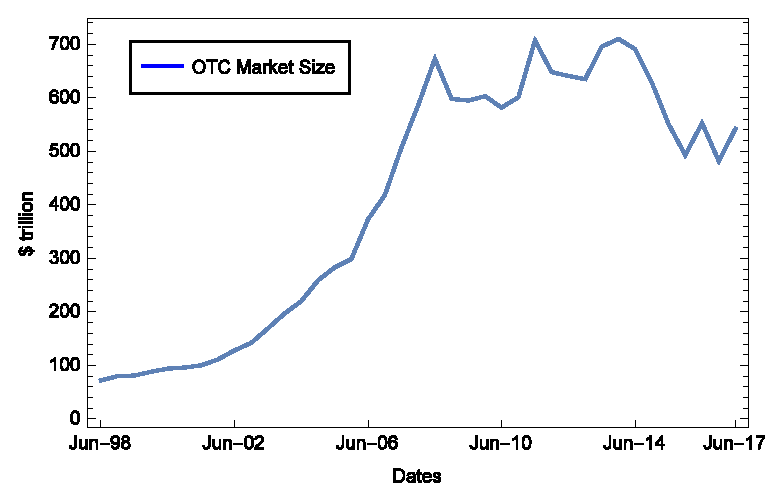
\includegraphics[width=1.0\columnwidth]{OTC.eps}
      \caption{Size of OTC derivatives market.\newline \footnotesize{\textbf{Source:} stats.bis.org/statx/srs/table/d5.1 (on 16/11/2017)}}\label{fig:OTC}
    \end{figure}


Among the many types of derivatives, the most commonly traded are options.

In simple terms, a \textit{call option} grants the investor the right to buy the underlying asset (e.g. stock) for a fixed price, known as the \textit{strike price}, by a certain date, known as the \textit{expiration date}.\\
On the other hand, a \textit{put option} grants the investor the right to sell the underlying asset for the strike price, by the expiration date.\\

\iffalse
Among these, the most commonly traded are call and put options. In short, a call (resp. put) option gives an investor the right to buy (resp. sell) a particular stock for a fixed price (called the strike price) at some point in the future. If the stock price increases above (resp. decreases below) the fixed price, the investor can simply buy the said stock in the stock market for the lower fixed (resp. current) price, and sell it immediately after for the higher current (resp. fixed) price, earning the difference. If, otherwise, the stock price goes down (resp. up), then the option is worthless and the investor loses his investment.\\
The payoff functions can be easily deduced as
\begin{equation}\label{callput}
\begin{split}
&\text{Payoff}_\text{call}(t)=(K-S(t))^+;\\
&\text{Payoff}_\text{put}(t)=(S(t)-K)^+,
\end{split}
\end{equation}
\noindent where $K$ is the strike price and $S(t)$ is the stock price at the time of exercise, $t$.\fi

Options have several advantages that make them especially appealing to investors.\\
To hedgers (i.e. investors that want to limit their exposure to risk), options provide safety by fixing the future price of a stock. If this investor is afraid of a price crash, by buying put options he ensures that future losses are contained (though if the crash doesn't occur, the hedger loses his option investment).\\
To speculators (i.e. investors that take advantage of the uncertainty of future asset prices by betting on their outcome), options grant access to much larger profits when the market forecast proves true (though also greater losses when it doesn't). In short, options magnify consequences: a good result turns into a large profit whereas a bad prediction results in a loss of investment.

Because of these advantages, an investor has to pay a certain fee to acquire an option. This pricing problem is a fundamental concern to investors. If an option is under-priced by a seller, an informed investor can earn great profits by taking advantage of it.
The price of an option and what influences it will be the main focus of this work.


\iffalse
For one, they limit the exposure to risk, e.g. if the price of a given stock were to crash, stock holders would lose a serious amount of funds whereas the owner of a call option would only lose his smaller original investment. On the other hand, options can also lead to greater profits e.g. using the same example of the stock price crash, the owner of a put option could buy this option for the lower current price (after the crash) and sell it for the higher price, fixed at the time of acquisition, before the crash happened.

This type of derivatives also comes with its own caveats. The main disadvantage is the fact that options always deal with stock prices in the future, i.e one can never precisely anticipate how much will be earned, if anything at all. Thus, it's clear that accurately modeling the stock price is paramount when dealing with options.
\fi


\subsection{European and American Options}
Both call and put options can be further separated into several types. Among these European and American options are by far the most commonly traded.
The holder of an \textit{European option} can exert his right to buy/sell (call/put) the underlying assets, also known as \textit{exercising}, only at the specified expiration date.
An \textit{American option} can be exercised at any point up to this very same date.


\iffalse
Call and put options are also divided into different types. The two most commonly used are European and American options. An European option can only be exercised - buying/selling the stocks for the fixed stock price with a call/put option - at a fixed date in the future, whereas an American option can be exercised anytime up until that fixed date. The payoffs of each of these types of options is simply
\begin{equation}
\begin{split}
&\text{Payoff}_\text{European}=\text{Payoff}_\text{call/put}(T);\\
&\text{Payoff}_\text{American}=\text{Payoff}_\text{call/put}(t), \ \ \ \forall 0<t<T,
\end{split}
\end{equation}

\noindent where $\text{Payoff}_\text{call/put}(t)$ corresponds to the payoffs from equations \ref{callput} and $T$ corresponds the fixed exercise date of European options.
\fi

Due to their high importance, options have been studied in detail in the past.
Possibly the most important result in this field came from Robert Merton and Myron Scholes who earned the 1997 Nobel prize in Economics for developing a mathematical model to price European options - the famous Black-Scholes formula - still used nowadays, though with some modifications.

Pricing American options, however, poses a greater challenge. Because they can be exercised at any time, the underlying assets must be closely monitored so as to attempt to exercise at an optimal point.
Furthermore, unlike European options, no analytic pricing model currently exists for this type of derivatives. Several numerical models have been proposed in the past in an attempt to approximate the price of these options. These methods shall be discussed in detail in the following chapters.

American options are still nonetheless very much used by investors, so it is absolutely critical to understand which variables influence these types of derivatives and by what amount. With this knowledge, one can better prepare oneself to market changes and even mitigate potential risks.

\section{Objectives}
The main objective of this thesis is to study which factors affect the price of an option and in what extent.

We will begin by replicating the model developed by Longstaff and Schwartz to price American options. Their method is based upon a Monte Carlo generation of stock price paths with a set of market variables such as stock volatility and interest rate (using the Black-Scholes stochastic deferential equation). To these results, a least squares regression is then applied iteratively to generate an optimal stopping decision matrix with all the stock price paths generated.

With this method, we shall then apply a variation-based sensitivity analysis, as developed by Sobol and Saltelli. This analysis outputs a weight for each of the variables used that corresponds to their influence in the variance of the final option price.
Thus, if a variable has a large weight, its variance has a large impact in the variance of the option price.

As a next step, we shall modify the Longstaff-Schwartz method to closely resemble real-world stocks. We will, for example, implement the GARCH(1,1) model for the stock price volatility to account for daily changes on its value. We could also try to implement interest rate models for the same reason.
A further study of which models better suit our needs is still necessary.

Finally, we will apply our model to real-world stock prices, publicly available, and try to predict option prices.

\iffalse
First we will begin by simulating a large number of stocks, using the simple Black-Scholes formula to generate each path. The main point behind this method is to apply the Monte Carlo approach to the stock price which will be used later in the option pricing.
After generating all the paths, we shall attempt to replicate the method developed by Longstaff and Schwartz for pricing American options, using the results from the previous simulation.
Next, we will modify the initial simulations using more complex models that better replicate real-world stocks, such as varying volatility, varying interest rate. We shall further study which other factors influence the final price of an option.
We shall then apply a sensitivity analysis on the option price, using the model developed by Sobol and Saltelli.
\fi

\section{State of the art}


Models to price American options, derived from the results of Black and Scholes, have also been proposed, among which the work of Longstaff and Schwartz are paramount.


Nowadays, computers have become fundamental tools in the study of stock


\iffalse

\noindent Derivatives have become increasingly important in recent decades, with the sums currently handled in these markets amounting to several trillion dollars.\\
For this reason, it is of the utmost importance to be able to accurately predict the payoff of such contracts to correctly price them.\\
In this thesis we will study particularly the pricing of American options. These contracts are especially difficult to price due to the high uncertainty associated with optimal stopping.\\
Several methods have been suggested to achieve this goal, such as finite difference, but we shall use the procedure proposed by Longstaff et al., using Monte Carlo simulation and least-squares regression.\\
We will mainly focus on the sensitivity analysis of this pricing process, namely how the parameters’ volatility affects the final calculated price.\\
This analysis is particularly important due to the sometimes-large uncertainty associated with the parameters used. For this reason, we find that the least-squares approach is ideal under such conditions, since we expect it to be less sensitive to volatility than other methods.
\fi
\section{Objectives}

\section{State of the Art}

\section{Commented Bibliography}
\begin{itemize}
\item Hull, J. (2012). \textit{Options, futures, and other derivatives}. Boston: Prentice Hall.

\item Longstaff, F. A., \& Schwartz, E. S. (2001, January 1). Valuing American Options by Simulation: A Simple Least-Squares Approach. \textit{The Review of Financial Studies, 14}(1), 113-147.

\item Choe, G. H. (2016). \textit{Stochastic Analysis for Finance with Simulations}. Universitext. Springer International Publishing. 
\end{itemize}
\section{Timetable}

\iffalse
\section{Thesis Supervisors}
\begin{itemize}
  \item Cláudia Nunes Philippart, \ \ cnunes@math.tecnico.ulisboa.pt
  \item Rui Manuel Agostinho Dilão, \ \ ruidilao@tecnico.ulisboa.pt
  \item Claude Yves Cochet, \ \ claude.cochet@bnpparibas.com
\end{itemize}
\fi

\end{document}

